\documentclass[../../main.tex]{subfiles}

\begin{document}

Wir wissen bereits, dass Aussagen entweder \wahr\  oder \falsch\  sind.
In diesem Abschnitt widmen wir uns der Frage, wie man denn nun herausfinden kann, 
ob eine Aussage \wahr\  oder \falsch\  ist. 

Blöderweise ist das in manchen Fällen gar nicht so einfach oder manchmal sogar gar nicht möglich. Das nächste Beispiel zeigt Aussagen, für die es aus verschiedenen Gründen schwierig ist zu entscheiden, ob sie \wahr\  oder \falsch\  sind.

\todo{Besseres Bild für den wütenden Zauberer}
\begin{example}{Aussagen mit schwierig zu bestimmenden Wahrheitswert}
        \parpic[r]{
        
\includegraphics[width=0.1\textwidth]{images/wizard_angry_tmp.png}
    }

    Der Wahrheitswert der Aussage \statement{Der Zauberer ist schlecht gelaunt} hängt davon ab, zu welchem Zeitpunkt diese Aussage getätigt wird. Es gibt nämlich Tage an denen der Zauberer gut gelaunt ist, es gibt aber auch welche an denen er schlecht gelaunt ist.
    \\ \\
    Den Wahrheitswert Aussage \statement{Der Bart vom Zauberer ist nicht echt} könnte man zwar prinzipiell bestimmen, indem man eine Probe seines Barthaares nimmt, jedoch würde der Zauberer dies nicht zulassen (sein Bart ist ihm heilig!).
    \\ \\
    Die Aussage \statement{Der Zaubertrank ist giftig} hat zwar einen Wahrheitswert, jedoch hängt dieser davon ab, auf welchen Zaubertrank sich die Aussage bezieht.
\end{example}

Wir stellen also fest, dass es Aussagen gibt, über die wir nicht ohne weiteres entscheiden können, ob sie \wahr\  oder \falsch\ \  sind. Das Problem ist, dass der Wahrheitswert von manchen Aussagen vom Zeitpunkt der Aufstellung der Aussage abhängt oder der Wahrheitswert vom Kontext abhängt in der die Aussage gestellt wurde. Der Wahrheitswert mancher Aussagen ist zwar im Prinzip bestimmbar, wäre jedoch viel zu aufwendig.

Wir müssen uns also damit abfinden, dass wir im Allgemeinen nicht über den Wahrheitswert einer Aussage entscheiden können. Wir geben uns damit aber noch nicht zufrieden. Können wir zumindest herausfinden, welche Informationen wir mindestens benötigen, um den Wahrheitswert einer Aussage zu bestimmen?

\begin{example}{Atomare Aussagen}
Wir betrachten noch einmal zwei der Aussagen aus dem letzten Beispiel und verknüpfen diese mit \statement{und} zu einer neuen Aussage, die lautet:
\[\statement{Der Zauberer ist schlecht gelaunt und der Zaubertrank ist giftig}\]
Angenommen wir würden die Wahrheitswerte von den beiden kleineren Unteraussagen
\begin{enumerate}
    \item \statement{Der Zauberer ist schlecht gelaunt}
    \item \statement{Der Zaubertrank ist giftig}
\end{enumerate}
kennen, dann könnten wir daraus den Wahrheitswert der gesamten Aussage ableiten. Wüssten wir zum Beispiel, dass der Zauberer schlecht gelaunt ist und, dass der Zaubertrank giftig ist, dann wüssten wir, dass unsere Aussage \statement{Der Zauberer ist schlecht gelaunt und der Zaubertrank ist giftig} \wahr\  ist.
\\ \\
Können wir mit dem gleichen Prinzip auch den Wahrheitswert der beiden Unteraussagen ermitteln? Nein, denn diese beiden Unteraussagen enthalten keine Konnektoren mehr. Sie sind also nicht aus kleineren Aussagen zusammengesetzt. Solche Aussagen, die keine Konnektoren enthalten, nennt man \textbf{atomare Aussagen}.
\end{example}

Die Erkenntnisse aus dem letzten Beispiel lassen sich verallgemeinern. Tatsächlich sind die einzigen Informationen, die wir benötigen, um den Wahrheitswert einer Aussage zu bestimmen, die Wahrheitswerte gewisser Unteraussagen. Diese gewissen Unteraussagen sind die sogenannten \textbf{atomaren Aussagen}. Das sind Aussagen, die keine Konnektoren enthalten. \enquote{Atomar} kommt aus dem griechischen und heißt \enquote{unteilbar}.

\begin{definition} {Atomare Aussage}
Eine \textbf{Atomare Aussage} ist eine Aussage, die keine Konnektoren enthält.
\end{definition}

Im Folgenden erläutern wir, wie man für beliebige Aussagen den Wahrheitswert bestimmen kann, falls man bereits die Wahrheitswerte aller atomaren Aussagen dieser Aussage kennt. Wir gehen also davon aus, dass wir zumindest die Wahrheitswerte von atomaren Aussagen immer \enquote{geschenkt} bekommen.

Als Zwischenschritt zeigen wir dafür zunächst, wie wir mit den Wahrheitswerten von zwei beliebigen Aussagen $A$,$B$,
auf die Wahrheitswerte von $A \land B$, $A \lor B$, $A \implies B$, $A \iff B$ und $\lnot A$ schließen
können. Mit diesem Wissen können wir dann später ein Verfahren angeben, um unser eigentliches Ziel zu erreichen:
Von den Wahrheitswerten von atomaren Unteraussagen auf den Wahrheitswert der gesamten Aussage schließen.

\textbf{Wahrheitswerte von dem Konnektor \enquote{und}}:
Betrachten wir zunächst den Fall, dass wir eine Aussage vorliegen haben, die dadurch entstanden ist, dass wir zwei Aussagen durch den Konnektor \statement{und} verknüpft haben. Das Symbol für \statement{und} ist $\land$. 
Seien nun $A,B$ zwei beliebige Aussagen. Angenommen, wir kennen die Wahrheitswerte von $A$ und $B$, was ist dann nun der Wahrheitswert von $A \land B$?  $A \land B$ ist genau dann \wahr, wenn sowohl $A$ als auch $B$ \wahr\  ist. Ist also $A$ oder $B$ \falsch\  oder sind sogar beide \falsch\ , dann ist auch $A \land B$ \falsch\ .

\begin{example}{Wahrheitswerte von $\land$}
    Sei $S$ eine Abkürzung für die Aussage \statement{Der Zauberer ist schlecht gelaunt} und $G$ eine Abkürzung für \statement{Der Zaubertrank ist giftig}. Ist der Zauberer tatsächlich schlecht gelaunt ($S$ ist \wahr) und ist der Zaubertrank giftig ($G$ ist auch \wahr), dann ist $S \land G$ \wahr. 
    
    Ist aber entweder $S$ oder $G$ \falsch\  oder sind sogar beide \falsch\ , dann ist $S \land G$ auch \falsch\ . Das in einer Tabelle zusammengetragen, sieht wie folgt aus:
    
    \[\begin{array}{cc s c}\toprule
        S & G & S \land G\\\midrule
        \falsch   & \falsch   & \falsch  \\
        \falsch   & \wahr & \falsch\\
        \wahr & \falsch   & \falsch\\
        \wahr & \wahr & \wahr\\\bottomrule
    \end{array}\]
\end{example}

Wir halten jetzt das, was wir gerade formuliert haben, präzise in einer Definition fest.

\begin{definition} {Wahrheitswerte von $\land$}
    Sind $A,B$ Aussagen von denen der Wahrheitswert bekannt ist, dann ergibt sich der Wahrheitswert von $A \land B$ durch folgende Tabelle.
    \[\begin{array}{cc s c}\toprule
        A & B & A \land B\\\midrule
        \falsch   & \falsch   & \falsch  \\
        \falsch   & \wahr & \falsch\\
        \wahr & \falsch   & \falsch\\
        \wahr & \wahr & \wahr\\\bottomrule
    \end{array}\]
\end{definition}

\textbf{Wahrheitswerte von dem Konnektor \enquote{oder}}: Betrachten wir als nächstes den Fall, dass wir eine Aussage vorliegen haben, die dadurch entstanden ist, 
dass wir zwei Aussagen durch den Konnektor \statement{oder} verknüpft haben. Das Symbol für \statement{oder} ist $\lor$. Seien nun $A,B$ zwei beliebige Aussagen. 
Angenommen wir kennen die Wahrheitswerte von $A$ und $B$, wie lässt sich daraus der Wahrheitswert von $A \lor B$ ermitteln? $A \lor B$ ist genau dann \wahr, wenn mindestens eine der Aussagen $A,B$ \wahr\  ist. Insbesondere ist $A \lor B$ auch \wahr\  wenn $A$ und $B$ beide gleichzeitig \wahr\  sind. Der einzige Fall in dem  $A \lor B$ \falsch\  wird, ist, wenn sowohl $A$ als auch $B$ beide \falsch\  sind.

\begin{example}{Wahrheitswerte von $\lor$}
    Sei $S$ wieder die Abkürzung für die Aussage \statement{Der Zauberer ist schlecht gelaunt} und $G$ wieder die Abkürzung für \statement{Der Zaubertrank ist giftig}. Ist mindestens eine Aussage der Aussagen $S, G$  \wahr, dann ist $S \lor G$ \wahr. Ist also zum Beispiel der Zauberer nicht schlecht gelaunt ($S$ ist \falsch\ ), aber der Zaubertrank ist giftig ($G$ ist \wahr), dann ist $S \lor G$ \wahr. 
    
    $S \lor G$ kann nur \falsch\  werden, wenn der Zauberer nicht schlecht gelaunt ist ($S$ ist \falsch) und der Zaubertrank nicht giftig ist ($G$ ist \falsch). Wir tragen alle möglichen Fälle in einer Tabelle zusammen:
    
    \[\begin{array}{cc s c}\toprule
        S & G & S \lor G\\\midrule
        \falsch   & \falsch   & \falsch  \\
        \falsch   & \wahr & \wahr\\
        \wahr & \falsch   & \wahr\\
        \wahr & \wahr & \wahr\\\bottomrule
    \end{array}\]
\end{example}

Die nächste Definition hält noch einmal genau das fest, was wir gerade besprochen haben.

\begin{definition}{Wahrheitswerte von $\lor$}
    Seien $A,B$ Aussagen von denen der Wahrheitswert bekannt ist. Dann ergibt sich der Wahrheitswert von $A \lor B$ durch folgende Tabelle.
    \[\begin{array}{cc s c}\toprule
        A & B & A \lor B\\\midrule
        \falsch   & \falsch   & \falsch  \\
        \falsch   & \wahr & \wahr\\
        \wahr & \falsch   & \wahr\\
        \wahr & \wahr & \wahr\\\bottomrule
    \end{array}\]
\end{definition}

\textbf{Wahrheitswerte der Negation}: Den nächsten Fall, den wir betrachten, ist die Negation. Zur Erinnerung: Verneinen wir eine Aussage, dann ist das die Negation der ursprünglichen Aussage. Ist $A$ eine beliebige  Aussage, dann notieren wir die Negation von $A$ durch $\lnot A$. Eine Negation dreht den Wahrheitswert der Aussage um. Das heißt, wenn die Aussage \wahr\  ist, dann ist ihre Negation \falsch\  und ist eine Aussage \falsch\ , dann ist ihre Negation \wahr.

\begin{example}{Wahrheitswerte von $\lnot$}
Sei $G$ noch einmal die Abkürzung für die Aussage \statement{Der Zaubertrank ist giftig}. Ist $G$ \wahr, dann ist die Negation $\lnot G$ \falsch. Ist aber andersherum $G$ \falsch, dann ist $\lnot G$ \wahr. Die folgende Tabelle verdeutlicht dies.
    \[\begin{array}{c s c}\toprule
        G & \lnot G\\\midrule
        \falsch & \wahr\\
        \wahr & \falsch\\\bottomrule
    \end{array}\]
\end{example}

Wie zuvor, halten wir diese Erkenntnisse auch nochmal in einer Definition fest.

\begin{definition}{Wahrheitswerte von $\lnot$}
    Sei $A$ eine Aussage dessen Wahrheitswert bekannt ist. Dann ergibt sich der Wahrheitswert von $\lnot A$ durch folgende Tabelle.
    \[\begin{array}{c s c}\toprule
        A & \lnot A\\\midrule
        \falsch & \wahr\\
        \wahr & \falsch\\\bottomrule
    \end{array}\]
\end{definition}

\textbf{Wahrheitswerte von dem Konnektor \enquote{genau dann, wenn}}: Betrachten wir nun den Fall, dass wir zwei Aussagen mit dem Konnektor \statement{genau dann, wenn} verknüpft haben. Solch eine Verknüpfung haben wir Äquivalenz genannt. Das Symbol für den Konnektor \statement{genau dann, wenn} notieren wir durch $\iff$. Seien nun $A,B$ zwei beliebige Aussagen. Wir definieren, dass $A \iff B$ genau dann \wahr\  ist, wenn $A$ denselben Wahrheitswert wie $B$ besitzt. 

\begin{example}{Wahrheitswerte von $\iff$}
    Sei $F$ eine Abkürzung für die Aussage \statement{Der Zaubertrank verleiht Superkräfte} und $S$ wieder die Abkürzung für \statement{Der Zauberer ist schlecht gelaunt}. Verleiht zum Beispiel der Zaubertrank keine Superkräfte (also $F$ ist \falsch) und ist der Zauberer nicht gut gelaunt ($G$ ist \falsch), dann ist trotzdem $F \iff G$ \wahr, da $F$ und $G$ den gleichen Wahrheitswert besitzen. 
    
    Verleiht der Zaubertrank Superkräfte ($F$ ist \wahr) und ist der Zauberer schlecht gelaunt ($G$ ist \falsch), dann ist $F \iff G$ \falsch, da die Wahrheitswerte von $F$ und $G$ unterschiedlich sind. Die folgende Tabelle zeigt alle möglichen Fälle der Wahrheitswerte von $F$ und $G$ und wie sich daraus der Wahrheitswert von $F \iff G$ ergibt.
    
    \[\begin{array}{cc s c}\toprule
        F & G & F \iff G\\\midrule
        \falsch   & \falsch   & \wahr  \\
        \falsch   & \wahr & \falsch\\
        \wahr & \falsch   & \falsch\\
        \wahr & \wahr & \wahr\\\bottomrule
    \end{array}\]
\end{example}

Wir halten das Beschriebene wieder in einer Definition fest.

\begin{definition}{Wahrheitswerte von $\iff$}
    Sind $A,B$ Aussagen von denen der Wahrheitswert bekannt ist, dann ergibt sich der Wahrheitswert von $A \iff B$ durch folgende Tabelle.
    \[\begin{array}{cc s c}\toprule
        A & B & A \iff B\\\midrule
        \falsch   & \falsch   & \wahr  \\
        \falsch   & \wahr & \falsch\\
        \wahr & \falsch   & \falsch\\
        \wahr & \wahr & \wahr\\\bottomrule
    \end{array}\]
\end{definition}

\textbf{Wahrheitswerte von dem Konnektor \enquote{wenn, dann}}: 
Den letzten Fall, den wir betrachten, ist die Implikation. Wir schauen jetzt also wie sich die Wahrheitswerte einer Implikation ergeben, wenn wir die Wahrheitswerte der Bedingung und der Konsequenz der Implikation kennen. Zur Erinnerung: Das Symbol für die Implikation lautet: $\implies$ und sie steht für den Konnektor \enquote{\textbf{wenn, dann}}.
Seien $A,B$ wieder zwei beliebige  Aussagen. Um die gleich folgende Definition besser nachvollziehen zu können, interpretiert man die Aussage $A \implies B$ als ein Versprechen. Nur wenn dieses Versprechen explizit gebrochen wird, soll $A \implies B$ \falsch\  werden. Das Versprechen ist nun, dass wenn $A$ \wahr\  ist, dann muss auch $B$ \wahr. Wenn $A$ \falsch\  ist, dann ist dem Versprechen egal, was mit $B$ passiert. Das Versprechen wird also nur gebrochen, wenn $A$ \wahr\  ist, aber $B$ \falsch\  ist.

\begin{example}{Wahrheitswerte von $\implies$}
    Sei $G$ wieder die Abkürzung für die Aussage \statement{Der Zauberer ist schlecht gelaunt} und $F$ wieder die Abkürzung für \statement{Der Zaubertrank verleiht Superkräfte}. 
    Ist beispielsweise der Zauberer nicht gut gelaunt ($G$ ist \falsch) und der Zaubertrank verleiht auch keine Superkräfte ($F$ ist \falsch), dann ist $G \implies F$ \wahr, da hier das Versprechen nicht gebrochen wurde, dass wenn der Zauberer gut gelaunt ist, der Zaubertrank Superkräfte verleihen wird. 
    
    Dieses Versprechen wird nur gebrochen, wenn der Zauberer gut gelaunt ist ($G$ ist \wahr) aber trotzdem der Trank keine Superkräfte verleiht ($F$ ist \falsch). Dann ist $G \implies F$ \falsch\ . Die folgende Tabelle listet für alle möglichen Kombinationen der Wahrheitswerte von $F,G$ den Wahrheitswert von $G \implies F$ auf. 
    
    \[\begin{array}{cc s c}\toprule
        G & F & G \implies F\\\midrule
        \falsch   & \falsch   & \wahr  \\
        \falsch   & \wahr & \wahr\\
        \wahr & \falsch   & \falsch\\
        \wahr & \wahr & \wahr\\\bottomrule
    \end{array}\]
\end{example}

Wir halten wieder die Überlegungen zur Definition der Wahrheitswerte einer Implikation in einer konkreten Definition fest.

\begin{definition}{Wahrheitswerte von $\implies$}
    Sind $A,B$ Aussagen von denen der Wahrheitswert bekannt ist, dann ergibt sich der Wahrheitswert von $A \implies B$ durch folgende Tabelle.
       \[\begin{array}{cc s c}\toprule
        A & B & A \implies B\\\midrule
        \falsch   & \falsch   & \wahr  \\
        \falsch   & \wahr & \wahr\\
        \wahr & \falsch   & \falsch\\
        \wahr & \wahr & \wahr\\\bottomrule
    \end{array}\]
\end{definition}

Wir haben jetzt Konnektor für Konnektor Wahrheitswerte definiert. Wir haben insgesamt die Konnektoren $\land,\lor,\implies,\iff,\lnot$ behandelt. Die folgende Tabelle fasst nochmal alle vorangegangen Definitionen in einer Tabelle zusammen.
\begin{definition}{Wahrheitswerte aller Konnektoren}
\label{whw}
Seien $A,B$ zwei beliebige Aussagen. Der Wahrheitswert aller möglichen Verknüpfungen dieser beiden Aussagen ist dann wie folgt definiert.

    \[\begin{array}{cc s ccccc}\toprule
        A & B & A \land B & A\lor B & A\implies B & A\iff B & \lnot A\\\midrule
        \falsch & \falsch & \falsch & \falsch & \wahr & \wahr & \multirow{2}{*}{\wahr}\\
        \falsch & \wahr & \falsch & \wahr & \wahr & \falsch &  \\
         \wahr & \falsch & \falsch & \wahr & \falsch & \falsch & \multirow{2}{*}{\falsch}
        \\
        \wahr & \wahr & \wahr & \wahr & \wahr & \wahr & 
         \\\bottomrule
    \end{array}\]
\end{definition}

Zu Beginn dieses Kapitels wurde erwähnt, dass die Wahrheitswerte von atomaren Unteraussagen einer völlig beliebigen Aussage, die einzigen Informationen sind, die wir 
benötigen um den Wahrheitswert der Aussage zu ermitteln. Die Grundidee, um nun den Wahrheitswert zu ermitteln, ist die Folgende: Beginnend bei den atomaren Unteraussagen 
einer Aussage, können wir den Wahrheitswert von immer komplexer werdenden Unteraussagen folgern, bis wir den Wahrheitswert der gesamten Aussage kennen.
Wie das funktioniert, schauen wir uns jetzt an.

Tatsächlich ist die Vorgehensweise, die wir gleich zeigen, nichts neues und funktioniert völlig analog zu einem Verfahren, das man bereits im Schlaf beherrscht: 
Dem Auswerten von Termen. Das nächste Beispiel wiederholt dies und dröselt die Schritte, die man dabei vornimmt, auf.

\todo{abbildung tikzen}
\begin{example}{Termauswertung}
Stell dir vor deine Aufgabe ist es den Term $x \cdot (y - (z \cdot z))$ auszuwerten und du weißt, dass $x = 3$, $y = 7$ und  $z = 2$ ist.
Um den Wert von $x \cdot (y - (z \cdot z))$ heraufzufinden, wendet man folgende Schritte an.
\begin{enumerate}
    \item Ersetze die Variablen im Term durch ihre Werte:
    \[x \cdot (y - (z \cdot z)) \longmapsto 3 \cdot (7 - (2 \cdot 2)) \]
    \item Bis das Ergebnis bekannt ist, führe folgende Schritte aus:
        \begin{enumerate}
            \item Wähle einen Teilterm dessen Wert direkt bestimmt werden kann.
            \item Ersetze diesen Teilterm durch seinen Wert.
        \end{enumerate}
    \end{enumerate}
    
    Die nächste Abbildung zeigt genau dieses Vorgehen. Dabei ist in jeder Zeile blau markiert welcher Teilterm gewählt und dann ersetzt wurde.
    \begin{center}
        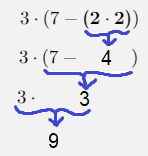
\includegraphics[width=0.275\textwidth]{images/TEMP_termalg.png}
    \end{center}

    Es bleibt am Ende nur noch 9 übrig. Wir haben damit herausgefunden, dass $x \cdot (y - (z \cdot z)) = 9$ ist.

\end{example}

Und genau diese Vorgehensweise, die wir beim Auswerten von Termen benutzen, lässt sich völlig analog auf das Auswerten von Aussagen übertragen. 
Es kommen nämlich genau dieselben Schritte vor. Möchte man nämlich den Wahrheitswert einer Aussage bestimmen, dann führt man folgende zwei Schritte aus:
    \begin{enumerate}
    \item Ersetze alle atomaren Aussagen durch ihren Wahrheitswert.
    \item 
        Wiederhole die nächsten beiden Teilschritte, bis nur noch ein Wahrheitswert übrig bleibt - Das Ergebnis.
        \begin{enumerate}
            \item Wähle einen einzelnen Wahrheitswert oder ein Paar von Wahrheitswerten, das durch einen Konnektor verknüpft ist.
            \item Ersetze den/die ausgewählten Wahrheitswert(e) durch den vom Konnektor vorgeschriebenen Wahrheitswert. Beispielsweise ersetzt man $\wahr \land \wahr$ durch $\wahr$ oder $\neg \wahr$ durch $\falsch$. 
        \end{enumerate}
    \end{enumerate}
    
Jetzt mal ein Beispiel in dem dieses Verfahren angewendet wird.

\todo{die abbildung tikzen}
\begin{example}{Wahrheiswertbestimmung}
Seien $A, B, C$ drei atomare Aussagen. Wenn wir wissen, dass $A$ \wahr\  ist, $B$ \wahr\  ist und $C$ \falsch\   ist, was ist dann der Wahrheitswert folgender Aussage?
\[A \land ( (\lnot B) \lor C)\]
Wir wenden das eben beschriebene, 2-schrittige Verfahren an.
\begin{enumerate}
    \item Zunächst ersetzen wir alle atomaren Aussagen durch ihren Wahrheitswert:
    \[A \land ( (\lnot B) \lor C) \longmapsto  \wahr \land ((\lnot \wahr) \lor \falsch)\]
    \item Solange bis nur noch ein einzelner Wahrheitswert übrig bleibt müssen wir jetzt also a) Paare oder einzelne Wahrheitswerte, die direkt mit einem Konnektor verknüpft sind, auswählen b) und durch den, vom Konnektor vorgeschriebenen, Wahrheitswert ersetzen.
    
    Die nächste Abbildung zeigt dieses Vorgehen nun in Aktion. In jeder Zeile ist dabei blau gekennzeichnet, welcher Wahrheitswert bzw. welches Paar von Wahrheitswerten gewählt und dann ersetzt wurde. 
\end{enumerate}
\begin{center}
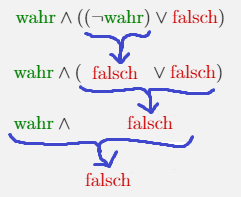
\includegraphics[width=0.4\textwidth]{images/TEMP_wahrheitsalg.png}
\end{center}
Es bleibt nur noch \falsch\  übrig. Es handelt sich dabei um den gesuchten Wahrheitswert. Insgesamt folgt also, dass $A \land ( (\lnot B) \lor C)$, \falsch\  ist.
\end{example}
Sei $A$ eine Aussage von der wir die Wahrheitswerte ihrer atomaren Unteraussagen kennen.
Wir wissen jetzt also wie wir von $A$ den Wahrheitswert ermitteln können. Kennt man die Wahrheitswerte der atomaren Unteraussagen aber nicht, kann man $A$ trotzdem analysieren indem man für alle Kombinationen der möglichen Wahrheitswerte der atomaren Unteraussagen, den Wahrheitswert von $A$ angibt.

Listen wir alle Kombinationen der Wahrheitswerte der atomaren Aussagen von $A$, zusammen mit den entsprechenden Wahrheitswerten von $A$ tabellarisch auf, dann nennen wir dies eine \textbf{Wahrheitstabelle} für $A$. 

\begin{example}{Wahrheitstabelle}
Wir stellen eine Wahrheitstabelle für die Aussage 
$A \land ( (\lnot B) \lor C)$
aus letztem Beispiel auf.
Die Aussage enthält die atomaren Aussagen $A,B,C$. Wir müssen also alle möglichen Kombinationen der Wahrheitswerte dieser auflisten. Dies sind 8 in der Zahl. Die Wahrheitstabelle der Aussage ist die folgende Tabelle. In der Tabelle sind als Hilfestellung noch die Wahrheitswerte aller Unteraussagen für jede Variablenbelegung angegeben. Das wäre aber nicht nötig gewesen. Die 7. Zeile entspricht den Wahrheiswerten, die wir im letzten Beispiel verwendet haben. 
    \[\begin{array}{ccc s ccc}\toprule
        A & B & C & \lnot B & (\lnot B) \lor C&A \land (\lnot B \lor C)\\\midrule
        \falsch & \falsch & \falsch &  \wahr& \wahr&\falsch \\
        \falsch & \falsch & \wahr &  \wahr& \wahr &\falsch \\
        \falsch & \wahr & \falsch & \falsch& \falsch &\falsch \\
        \falsch & \wahr & \wahr &\falsch & \wahr &\falsch \\
        \wahr & \falsch & \falsch &  \wahr& \wahr &\wahr \\
        \wahr & \falsch & \wahr & \wahr & \wahr &\wahr \\
        \wahr & \wahr & \falsch & \falsch& \falsch&\falsch \\
        \wahr & \wahr & \wahr & \falsch& \wahr &\wahr \\
        \bottomrule
    \end{array}\]
\end{example}

Die nächste Definition formalisiert das eben beschriebene Konzept von Wahrheitstabellen. Dort wird allgemein definiert, was für eine beliebige Aussage die zugehörige Wahrheitstabelle ist.

\begin{definition}{Wahrheitstabelle}
Ist $A$ eine Aussage und kommen in $A$ die atomaren Unteraussagen $x_1,\dots,x_n$ vor, dann nennen wir eine Tabelle, die für alle möglichen Kombinationen der Wahrheitswerte von $x_1,\dots,x_n$ den Wahrheitswert von $A$ angibt, eine \textbf{Wahrheitstabelle} für $A$.
\end{definition}

Prinzipiell kann man nach dieser Definition für jede Aussage eine Wahrheitstabelle aufstellen. In der Praxis gibt es aber Aussagen für die das aber nicht unbedingt sinnvoll ist, da die Wahrheitswerte der atomaren Aussagen offensichtlich sind und es sich daher nicht lohnt Fälle durchzuspielen, in denen die atomaren Aussagen andere Wahrheitswerte annehmen. Das könnte ja eh nicht eintreten. Ein Beispiel hierfür ist die Aussage: \statement{1 ist gleich 1 oder 1 ist gleich 1}. Den Fall durch zuspielen, dass \statement{1 ist gleich 1}, \falsch\ ist, wäre zwar prinzipiell möglich, ist aber wenig sinnvoll. 

Wir wollen jetzt unser neu gewonnenes Wissen nutzen, um das Logikrätsel aus 
der Einleitung systematisch zu lösen.

\begin{example}{Lösung Logikrätsel}
    \parpic[r]{
        
\includegraphics[width=0.2\textwidth]{images/wizard.png}
    }
    
    Wiederholung des Rätsels: \textit{Ein Zauberer gibt dir einen Zaubertrank, 
    der entweder giftig ist oder dir Flügel verleiht. Der Zauberer sagt entweder 
    immer die Wahrheit oder lügt immer.}
    
    \textit{Er gestattet dir \emph{eine} Frage, um herauszufinden, ob der 
    Zaubertrank giftig ist oder dir Flügel verleiht.}
    
    \picskip{1}
     \textbf{Welche Frage musst du dem Zauberer also stellen, um herauszufinden, ob der Trank giftig ist?}
    
    Lösung des Rätsels: Wir können die Gesamtsituation auch so auffassen, dass 
    wir dem Zauberer
    eine Aussage nennen. Wenn der Zauberer die Wahrheit sagt, dann nennt er uns den 
    echten
    Wahrheitswert der Aussage
    und wenn der Zauberer lügt, dann nennt er uns nicht den echten
     Wahrheitswert der Aussage, sondern den falschen. Wir tragen einmal in einer Tabelle die verschiedenen
     Fälle zusammen, die auftreten können. $A$ steht dabei für den echten Wahrheitswert
     unser Aussage (die wir jetzt noch nicht kennen), $L$ dafür, ob der Zauberer
     lügt und $AZ$ für den Wahrheitswert, den uns der Zauberer nennt. 
    
     \[\begin{array}{cc s c}\toprule
        A & L & AZ\\\midrule
        \falsch & \falsch &\falsch  \\
        \falsch & \wahr &\wahr  \\
        \wahr & \falsch &\wahr  \\
        \wahr & \wahr &\falsch  \\
        \bottomrule
    \end{array}\]

    Wir wollen unsere Aussage so wählen, dass wir mit dem Wahrheitswert, den uns 
    der Zauberer
    nennt, darauf rückschließen können, ob der Trank giftig ist. Konkret: Ist der Trank
    giftig, dann wollen wir dass der Wahrheitswert vom Zauberer \wahr\  ist und wenn der Trank
    Flügel verleiht (also nicht giftig ist), dann soll der Wahrheitswert vom Zauberer \falsch\  sein, unabhängig
    davon ob der Zauberer lügt oder nicht. Wir halten diese Forderung in einer Tabelle fest.
    $G$ steht für \statement{Giftig} und $L$, $AZ$ wie oben.

    \[\begin{array}{cc s c}\toprule
        G & L & AZ\\\midrule
        \falsch & \falsch & \falsch  \\
        \falsch & \wahr & \falsch  \\
        \wahr & \falsch & \wahr  \\
        \wahr & \wahr & \wahr  \\
        \bottomrule
    \end{array}\]

    Daraus können wir bereits schließen, welche Wahrheitswerte, die Aussage
    haben muss, die wir dem Zauberer nennen in Abhängigkeit von $G$,$L$. 
    Wir müssen dazu nämlich nur die Wahrheitswerte in den Fällen umdrehen, in denen der 
    Zauberer lügt. Im Fall $G$ \falsch\ und $L$ \wahr\  wollen wir zum Beispiel, dass
    die Antwort vom Zauberer \falsch\ ist. Da der Zauberer aber lügt, muss unsere
    Aussage in diesem Fall also \wahr\ sein.
    
    Wir ergänzen die letzte Tabelle jetzt also um die Spalte $A$, die
    die Wahrheitswerte enthält, die unsere Aussage haben muss.

    \[\begin{array}{cc s cc}\toprule
        G & L & A &AZ\\\midrule
        \falsch & \falsch & \falsch &\falsch  \\
        \falsch & \wahr & \wahr &\falsch  \\
        \wahr & \falsch & \wahr &\wahr  \\
        \wahr & \wahr & \falsch &\wahr  \\
        \bottomrule
    \end{array}\]

    Denkt man sich die Spalte $AZ$ weg, dann ist die letzte Tabelle eine Wahrheitstabelle
    für die Aussage, die wir dem Zauberer nennen wollen. Wir müssen jetzt also nur
    noch eine Aussage finden, die zu dieser Wahrheitstabelle passt.
    Das kriegen wir hin, indem wir uns anschauen in welchen Fällen, die Aussage \wahr\  sein soll.
    Die Aussage, die wir suchen, sagt dann aus, ob mindestens einer dieser Fälle eintritt.
    Konkret: Die Fälle, in denen die Aussage \wahr\  werden soll sind 1. $G$ 
    \falsch\ , $L$ \wahr\ 2.
    $G$ \wahr\ , $L$ \falsch. Dass der 1. Fall eintritt, formulieren wir durch
    $\lnot G \land L$ und dass der 2. Fall eintritt durch $G \land \lnot L$. 
    Und dass mindestens einer dieser Fälle eintritt durch
    \[ (\lnot G \land L) \lor (G \land \lnot L)\]
    Das ist genau die Aussage die wir gesucht haben und damit auch die Lösung unseres
    Rätsels. Natürlichsprachlich formuliert, würden wir den Zauberer also fragen:

    \textbf{(Ist der Trank nicht giftig und lügst du) oder (ist der Trank giftig und lügst du nicht) ?}
    
    Egal ob der Zauberer nun lügt oder nicht, wir haben diese Frage bzw. Aussage so konstruiert,
    dass der Zauberer mit \textit{Nein}, bzw. \falsch\ antworten wird, wenn 
    der Trank nicht giftig ist
    und mit \textit{Ja}, bzw. \wahr\ antworten wird, wenn der Trank
    giftig ist.

\end{example}

\begin{nutshell}{Wahrheitstabellen}
    Eine \textbf{atomare Aussage} ist eine Aussage, die keine Konnektoren enthält. \bigskip
   
    Eine \textbf{Wahrheitstabelle} einer Aussage gibt für alle möglichen Kombinationen der Wahrheitswerte der atomaren Unteraussagen an, was der Wahrheitswert der Aussage ist.\bigskip

    Seien $A,B$ beliebige Aussagen. Die folgende Tabelle definiert für alle Konnektoren den Wahrheitswert der Verknüpfung von $A,B$.
    \[\begin{array}{cc s ccccc}\toprule
        A & B & A \land B & A\lor B & A\implies B & A\iff B & \lnot A\\\midrule
        \falsch & \falsch & \falsch & \falsch & \wahr & \wahr & \multirow{2}{*}{\wahr}\\
        \falsch & \wahr & \falsch & \wahr & \wahr & \falsch &  \\
         \wahr & \falsch & \falsch & \wahr & \falsch & \falsch & \multirow{2}{*}{\falsch}
        \\
        \wahr & \wahr & \wahr & \wahr & \wahr & \wahr & 
         \\\bottomrule
    \end{array}\]
    \\ \\
    Möchte man den Wahrheitswert einer Aussage bestimmen und kennt man die Wahrheitswerte ihrer atomaren Aussagen, dann geht man wie folgt vor:
    \begin{enumerate}
    \item Ersetze alle atomaren Aussagen durch ihren Wahrheitswert.
    \item 
        Wiederhole die nächsten beiden Teilschritte, bis nur noch ein Wahrheitswert übrig bleibt - Das Ergebnis.
        \begin{enumerate}
            \item Wähle einen einzelnen Wahrheitswert oder ein Paar von Wahrheitswerten, das durch einen Konnektor verknüpft ist.
            \item Ersetze den/die ausgewählten Wahrheitswert(e) durch den vom Konnektor vorgeschriebenen Wahrheitswert. 
        \end{enumerate}
    \end{enumerate}

\end{nutshell}

\end{document}
